% =====================================================================
% Archivo: AreasdeOportunidadCEL.tex
% Propósito: Documento "Áreas de Oportunidad del Sistema CEL"
% Estilo: Español institucional (México) con clase cel.cls
% Integración: Guía horizontal y mejores prácticas SENER
% =====================================================================

\documentclass{cel}

% --- Metadatos del Documento ---
\title{Áreas de Oportunidad del Sistema de Certificados de Energía Limpia (CEL)}
\subtitle{Análisis Integral y Propuestas de Modernización}
\author{SENER}
\date{\today}
\institucion{Secretaría de Energía (SENER)}
\unidad{Unidad de Planeación Energética}
\setDocumentoCorto{Áreas CEL}
\palabrasclave{Energía, CEL, Certificados, Modernización}
\version{1.0}

% --- Metadatos PDF/UA (Accesibilidad Universal) ---
\hypersetup{
  pdftitle={Áreas de Oportunidad del Sistema de Certificados de Energía Limpia (CEL)},
  pdfauthor={SENER},
  pdfsubject={Sistema CEL - Áreas de Oportunidad},
  pdfkeywords={Energía, CEL, Certificados, Modernización, Sistema},
  pdfversion={1}
}

\begin{document}

% Portada institucional con fondo personalizado
\portadafondo[img/portada.png]

% Página de créditos/directorio
\paginacreditos{
\begin{center}
{\Large\bfseries\color{gobmxGuinda} Directorio}\\[1cm]
\end{center}

\vspace{1cm}

\begin{center}
{\large\bfseries\color{senerGuindaOscuro} Secretaría de Energía}\\[0.5cm]
{\normalsize Luz Elena González Escobar}\\
{\small\color{gobmxGris} Secretaria de Energía}\\[1cm]

{\large\bfseries\color{senerGuindaOscuro} Unidad de Planeación Energética}\\[0.5cm]
{\normalsize Dr. Leonardo Beltrán Rodríguez}\\
{\small\color{gobmxGris} Titular de la Unidad de Planeación Energética}\\[1cm]

{\large\bfseries\color{senerGuindaOscuro} Comisión Nacional de Energía}\\[0.5cm]
{\normalsize Ing. Arturo Herrera Gutiérrez}\\
{\small\color{gobmxGris} Comisionado Presidente}\\[1cm]

{\large\bfseries\color{senerGuindaOscuro} Equipo Técnico}\\[0.5cm]
{\normalsize Dirección General de Planeación e Información Energéticas}\\
{\normalsize Dirección General de Electricidad}\\
{\normalsize Dirección de Energías Limpias}\\
\end{center}
}

% Índice General (TOC)
{
  \hypersetup{linkcolor=gobmxGuinda}
  \tableofcontents
}
\newpage

% =====================================================================
% INTRODUCCIÓN
% =====================================================================
\phantomsection
\addcontentsline{toc}{section}{Introducción}
\section*{Introducción}

El Sistema de Certificados de Energía Limpia (S-CEL) constituye uno de los instrumentos centrales de la política de transición energética de México. Establecido en el marco de la Ley del Sector Eléctrico y operado mediante las Disposiciones Administrativas de Carácter General emitidas por la Comisión Nacional de Energía (CNE), este sistema busca incentivar la generación de energía limpia y garantizar el cumplimiento de las metas nacionales de energías limpias.

Sin embargo, la implementación operativa del S-CEL a lo largo de los últimos años ha revelado áreas de oportunidad significativas que requieren atención integral. El presente documento identifica, analiza y propone soluciones sistémicas para modernizar y optimizar el funcionamiento del sistema, con un enfoque jurídico-operativo que garantice la eficiencia, transparencia y cumplimiento de los objetivos de política energética nacional.

El análisis se estructura en bloques temáticos que abordan desde los procesos de entrada al sistema hasta los mecanismos de cumplimiento y sanción, proporcionando para cada área:

\begin{itemize}
    \item Diagnóstico de la situación actual
    \item Identificación de brechas y oportunidades
    \item Propuestas de mejora normativa y operativa
    \item Beneficios esperados de la implementación
\end{itemize}

Este documento se enmarca en el contexto de la Nueva Ley del Sector Eléctrico (2025) y la reconfiguración institucional del sector energético, buscando posicionar al S-CEL como un sistema de vanguardia que contribuya efectivamente a la soberanía energética y la transición hacia un modelo energético más limpio y sustentable.

\newpage

% =====================================================================
% BLOQUE I · ENTRADA AL SISTEMA Y BASE OPERATIVA
% =====================================================================

% Portada de sección para Bloque I
\portadaseccion{I}{Entrada al Sistema y Base Operativa}{Procesos de inscripción, registro y administración del S-CEL}

\section{Proceso de inscripción al Sistema de Certificados de Energía Limpia (S-CEL)}

% ----------------- PARTE A -----------------
\subsection{Tabla de validación jurídica (interna)}

El proceso de inscripción al S-CEL presenta diversas complejidades normativas que requieren análisis detallado para identificar oportunidades de mejora.

\begin{tabladoradoLargo}
    \tiny
    \begin{xltabular}{\textwidth}{|p{3.2cm}|p{3.5cm}|p{4.7cm}|p{2.5cm}|p{3.5cm}|}
    \caption{Matriz de Validación Jurídica - Proceso de Inscripción} \label{tab:validacion_inscripcion} \\
    \toprule
    \rowcolor{gobmxDorado} 
    \encabezadodorado{Hallazgo} & 
    \encabezadodorado{Instrumento (art./num.)} & 
    \encabezadodorado{Cita textual} & 
    \encabezadodorado{Riesgo} & 
    \encabezadodorado{Ajuste propuesto} \\
    \midrule
    \endhead
    
    \textbf{Complejidad documental excesiva} & 
    DACG S-CEL (RES/174/2016), Disp. 15 & 
    "Los Generadores Limpios deberán presentar... la documentación que acredite el cumplimiento de los requisitos..." & 
    Operativo: Barreras de entrada que limitan participación & 
    Simplificar requisitos documentales y digitalizar procesos \\
    \hline
    
    \textbf{Plazos de respuesta indefinidos} & 
    DACG S-CEL (RES/174/2016), Disp. 16 & 
    "La Comisión revisará la solicitud y documentación..." & 
    Jurídico: Incertidumbre sobre tiempos de resolución & 
    Establecer plazos máximos de respuesta (30 días hábiles) \\
    \hline
    
    \textbf{Criterios de evaluación subjetivos} & 
    DACG S-CEL (RES/174/2016), Disp. 17 & 
    "La Comisión podrá requerir información adicional..." & 
    Regulatorio: Discrecionalidad excesiva en evaluación & 
    Definir criterios objetivos y exhaustivos de evaluación \\
    \hline
    
    \textbf{Falta de mecanismo de apelación} & 
    DACG S-CEL (RES/174/2016) & 
    No se establece procedimiento de recurso & 
    Jurídico: Indefensión ante resoluciones negativas & 
    Implementar procedimiento de recurso de revisión \\
    \bottomrule
    \end{xltabular}
\end{tabladoradoLargo}

% ----------------- PARTE B -----------------
\subsection{Fuentes de información del S-CEL (obligatorio)}

\begin{tabladoradoLargo}
    \tiny
    \begin{xltabular}{\textwidth}{|p{2.5cm}|p{3cm}|p{2cm}|p{5cm}|}
    \caption{Fuentes de Información del S-CEL - Inscripción} \label{tab:fuentes_inscripcion} \\
    \toprule
    \rowcolor{gobmxDorado} 
    \encabezadodorado{Actor/Fuente} & 
    \encabezadodorado{Instrumento} & 
    \encabezadodorado{Artículo/Numeral} & 
    \encabezadodorado{Cita explícita} \\
    \midrule
    \endhead
    
    \textbf{Generadores Limpios} & 
    DACG S-CEL (RES/174/2016) & 
    Disp. 15 & 
    "Los Generadores Limpios deberán presentar solicitud de inscripción..." \\
    \hline
    
    \textbf{CNE} & 
    DACG S-CEL (RES/174/2016) & 
    Disp. 16 & 
    "La Comisión revisará la solicitud y documentación presentada..." \\
    \hline
    
    \textbf{Unidades de Inspección} & 
    RES/2910/2017 & 
    Anexo 1 & 
    "Certificación de la medición de variables para determinar el porcentaje de ELC" \\
    \hline
    
    \textbf{CENACE} & 
    DACG S-CEL (RES/174/2016) & 
    Disp. 26 & 
    "Informarán a la Comisión mediante el Sistema..." \\
    \bottomrule
    \end{xltabular}
\end{tabladoradoLargo}

\subsection{Diagnóstico de la situación actual}

El proceso de inscripción al S-CEL presenta las siguientes problemáticas principales:

\begin{enumerate}
    \item \textbf{Complejidad Administrativa}: El proceso requiere múltiples documentos y validaciones que pueden tomar meses en completarse.
    \item \textbf{Falta de Digitalización}: La mayoría de trámites se realizan en formato físico, generando ineficiencias.
    \item \textbf{Criterios Ambiguos}: Los requisitos de evaluación no están completamente objetivados.
    \item \textbf{Ausencia de Ventanilla Única}: Los solicitantes deben interactuar con múltiples instancias.
\end{enumerate}

\subsection{Estado objetivo}

El estado objetivo busca establecer un proceso de inscripción:

\begin{itemize}
    \item \textbf{Digitalizado}: Plataforma en línea con seguimiento en tiempo real
    \item \textbf{Eficiente}: Plazos máximos definidos y respetados
    \item \textbf{Transparente}: Criterios objetivos y públicos
    \item \textbf{Accesible}: Reducción de barreras de entrada
\end{itemize}

\subsection{Tabla comparativa: modelo actual vs modelo objetivo}

\begin{tabladoradoCorto}
  \caption{Comparativa: Proceso de Inscripción}
  \begin{tabularx}{\textwidth}{L{0.25\textwidth} X X}
    \toprule
    \rowcolor{gobmxDorado} 
    \encabezadodorado{Concepto} & 
    \encabezadodorado{Modelo Actual} & 
    \encabezadodorado{Modelo Objetivo} \\
    \midrule
    
    \textbf{Modalidad} & 
    Presencial/físico con documentos impresos & 
    Digital con firma electrónica avanzada \\
    
    \textbf{Plazos} & 
    Indefinidos, sujetos a disponibilidad & 
    Máximo 30 días hábiles con notificaciones automáticas \\
    
    \textbf{Seguimiento} & 
    Manual, requiere consultas telefónicas & 
    Plataforma en línea con estatus en tiempo real \\
    
    \textbf{Criterios} & 
    Subjetivos, sujetos a interpretación & 
    Objetivos, automatizados donde sea posible \\
    
    \textbf{Recursos} & 
    No existe mecanismo formal de apelación & 
    Recurso de revisión en línea con plazos definidos \\
    \bottomrule
  \end{tabularx}
\end{tabladoradoCorto}

\subsection{Arquitectura del sistema (alto nivel)}

La nueva arquitectura del proceso de inscripción se basará en:

\begin{enumerate}
    \item \textbf{Portal de Inscripción Digital}: Interfaz web responsiva con validaciones en tiempo real
    \item \textbf{Motor de Validación Automática}: Sistema que verifica documentos y requisitos automáticamente
    \item \textbf{Base de Datos Integrada}: Conexión con registros de CNE, CENACE y otras dependencias
    \item \textbf{Sistema de Notificaciones}: Alertas automáticas por correo y SMS
    \item \textbf{Panel de Control}: Dashboard para seguimiento de solicitudes
\end{enumerate}

\subsection{Reingeniería de procesos (pasos operativos)}

\textbf{Proceso Mejorado de Inscripción:}

\begin{enumerate}
    \item \textbf{Registro en Portal}: El solicitante crea cuenta con FIEL
    \item \textbf{Captura de Información}: Formulario inteligente con validaciones
    \item \textbf{Carga de Documentos}: Upload con verificación automática de formatos
    \item \textbf{Validación Automática}: Sistema verifica requisitos básicos
    \item \textbf{Revisión Técnica}: Personal especializado revisa casos complejos
    \item \textbf{Resolución}: Notificación automática de resultado
    \item \textbf{Recurso (si aplica)}: Proceso de apelación en línea
\end{enumerate}

\subsection{Beneficios esperados}

\begin{enumerate}
    \item \textbf{Reducción de Tiempos}: De meses a máximo 30 días hábiles
    \item \textbf{Mayor Transparencia}: Seguimiento en tiempo real del proceso
    \item \textbf{Reducción de Costos}: Eliminación de trámites presenciales
    \item \textbf{Mejor Experiencia}: Interfaz amigable y moderna
    \item \textbf{Incremento en Participación}: Menores barreras de entrada
    \item \textbf{Trazabilidad Completa}: Registro histórico de todas las acciones
\end{enumerate}

\subsection{Propuesta de ajuste normativo}

\begin{glowBox}[gobmxDorado]{Propuesta de Modificación Normativa}
\textbf{Disposición 15 Bis (Adición):}
"Proceso Digital de Inscripción. La inscripción al S-CEL se realizará exclusivamente a través del portal digital oficial, utilizando firma electrónica avanzada. El sistema proporcionará seguimiento en tiempo real y notificaciones automáticas del estatus de la solicitud."

\textbf{Disposición 16 (Modificación):}
"Plazos de Resolución. La Comisión resolverá las solicitudes de inscripción en un plazo máximo de treinta días hábiles contados a partir de la presentación completa de la documentación. Transcurrido este plazo sin resolución, la solicitud se tendrá por aprobada."

\textbf{Disposición 17 Bis (Adición):}
"Recurso de Revisión. Contra las resoluciones de inscripción procederá recurso de revisión ante la propia Comisión, el cual deberá interponerse dentro de los quince días hábiles siguientes a la notificación, a través del portal digital."
\end{glowBox}

% =====================================================================
\section{Registro de participantes, cuentas y administración del S-CEL}

\subsection{Tabla de validación jurídica (interna)}

\begin{tabladoradoLargo}
    \tiny
    \begin{xltabular}{\textwidth}{|p{3.2cm}|p{3.5cm}|p{4.7cm}|p{2.5cm}|p{3.5cm}|}
    \caption{Matriz de Validación Jurídica - Registro y Administración} \label{tab:validacion_registro} \\
    \toprule
    \rowcolor{gobmxDorado} 
    \encabezadodorado{Hallazgo} & 
    \encabezadodorado{Instrumento (art./num.)} & 
    \encabezadodorado{Cita textual} & 
    \encabezadodorado{Riesgo} & 
    \encabezadodorado{Ajuste propuesto} \\
    \midrule
    \endhead
    
    \textbf{Gestión manual de cuentas} & 
    DACG S-CEL (RES/174/2016), Disp. 18 & 
    "La Comisión asignará una cuenta a cada participante..." & 
    Operativo: Ineficiencia y errores en gestión manual & 
    Automatizar creación y gestión de cuentas \\
    \hline
    
    \textbf{Falta de interoperabilidad} & 
    DACG S-CEL (RES/174/2016) & 
    No se establece conexión con otros sistemas & 
    Técnico: Duplicidad de información y desactualización & 
    Implementar APIs de integración con sistemas externos \\
    \hline
    
    \textbf{Seguridad limitada} & 
    DACG S-CEL (RES/174/2016) & 
    Criterios de seguridad no especificados & 
    Seguridad: Vulnerabilidad a ataques cibernéticos & 
    Implementar estándares de ciberseguridad avanzados \\
    \bottomrule
    \end{xltabular}
\end{tabladoradoLargo}

\subsection{Fuentes de información del S-CEL (obligatorio)}

Las fuentes de información para el registro y administración incluyen datos de participantes, transacciones, y estados de cuenta que deben mantenerse actualizados y seguros.

\subsection{Diagnóstico de la situación actual}

El sistema actual de registro y administración presenta:

\begin{itemize}
    \item Procesos manuales propensos a errores
    \item Falta de integración con sistemas externos
    \item Limitaciones en la trazabilidad de transacciones
    \item Ausencia de herramientas de análisis avanzado
\end{itemize}

\subsection{Estado objetivo}

Implementar un sistema de administración moderno que incluya:

\begin{itemize}
    \item Gestión automatizada de cuentas y participantes
    \item Integración con sistemas de la CNE, CENACE y otras dependencias
    \item Trazabilidad completa de todas las operaciones
    \item Herramientas de análisis y reportes en tiempo real
\end{itemize}

\subsection{Tabla comparativa: modelo actual vs modelo objetivo}

\begin{tabladoradoCorto}
  \caption{Comparativa: Administración del Sistema}
  \begin{tabularx}{\textwidth}{L{0.25\textwidth} X X}
    \toprule
    \rowcolor{gobmxDorado} 
    \encabezadodorado{Concepto} & 
    \encabezadodorado{Modelo Actual} & 
    \encabezadodorado{Modelo Objetivo} \\
    \midrule
    
    \textbf{Gestión de Cuentas} & 
    Manual, propensa a errores & 
    Automatizada con validaciones en tiempo real \\
    
    \textbf{Integración} & 
    Sistemas aislados & 
    Interoperabilidad completa vía APIs \\
    
    \textbf{Seguridad} & 
    Básica, centrada en acceso & 
    Multicapa con encriptación y auditoría \\
    
    \textbf{Reportes} & 
    Manuales, con retrasos & 
    Automáticos, en tiempo real \\
    \bottomrule
  \end{tabularx}
\end{tabladoradoCorto}

\subsection{Arquitectura del sistema (alto nivel)}

La nueva arquitectura incluirá:

\begin{enumerate}
    \item \textbf{Microservicios}: Arquitectura modular y escalable
    \item \textbf{Base de Datos Distribuida}: Alta disponibilidad y respaldo
    \item \textbf{APIs RESTful}: Integración estándar con sistemas externos
    \item \textbf{Blockchain}: Para trazabilidad inmutable de transacciones
    \item \textbf{Analytics Engine}: Procesamiento de datos en tiempo real
\end{enumerate}

\subsection{Reingeniería de procesos (pasos operativos)}

\textbf{Proceso Automatizado de Administración:}

\begin{enumerate}
    \item \textbf{Registro Automático}: Creación de cuentas al completar inscripción
    \item \textbf{Sincronización}: Actualización automática con sistemas externos
    \item \textbf{Monitoreo Continuo}: Alertas automáticas de anomalías
    \item \textbf{Respaldo Automático}: Copias de seguridad programadas
    \item \textbf{Auditoría Continua}: Registro inmutable de todas las operaciones
\end{enumerate}

\subsection{Beneficios esperados}

\begin{enumerate}
    \item \textbf{Eficiencia Operativa}: Reducción significativa de errores manuales
    \item \textbf{Seguridad Mejorada}: Protección avanzada contra amenazas
    \item \textbf{Transparencia Total}: Trazabilidad completa de operaciones
    \item \textbf{Escalabilidad}: Capacidad de crecimiento sin degradación
    \item \textbf{Interoperabilidad}: Integración fluida con ecosistema digital
\end{enumerate}

\subsection{Propuesta de ajuste normativo}

Se requiere actualizar las disposiciones para reflejar la modernización tecnológica y establecer estándares de seguridad y operación.

% =====================================================================
\section{Medición, fuentes de información y datos vinculantes}

\subsection{Tabla de validación jurídica (interna)}

La medición constituye el fundamento técnico del S-CEL, por lo que requiere análisis detallado de sus bases normativas.

\subsection{Fuentes de información del S-CEL (obligatorio)}

Las fuentes incluyen expresamente: CENACE, Transportistas, Distribuidores, y reportes de Participantes Obligados (abasto aislado interconectado/no interconectado).

\subsection{Diagnóstico de la situación actual}

El sistema actual presenta limitaciones en:

\begin{itemize}
    \item Cobertura parcial de la generación distribuida
    \item Falta de integración del abasto aislado
    \item Dependencia de reportes manuales
    \item Ausencia de validación cruzada automática
\end{itemize}

\subsection{Estado objetivo}

Implementar un sistema de medición universal que capture toda la generación limpia del país, independientemente de su escala o modalidad de conexión.

\subsection{Tabla comparativa: modelo actual vs modelo objetivo}

\begin{tabladoradoCorto}
  \caption{Comparativa: Sistema de Medición}
  \begin{tabularx}{\textwidth}{L{0.25\textwidth} X X}
    \toprule
    \rowcolor{gobmxDorado} 
    \encabezadodorado{Concepto} & 
    \encabezadodorado{Modelo Actual} & 
    \encabezadodorado{Modelo Objetivo} \\
    \midrule
    
    \textbf{Cobertura} & 
    Limitada a gran escala interconectada & 
    Universal: gran escala + distribuida + aislada \\
    
    \textbf{Fuentes de Datos} & 
    Principalmente CENACE & 
    CENACE + Distribuidores + IoT + Telemetría \\
    
    \textbf{Validación} & 
    Manual, ex-post & 
    Automática, en tiempo real \\
    
    \textbf{Trazabilidad} & 
    Limitada & 
    Completa, desde generación hasta consumo \\
    \bottomrule
  \end{tabularx}
\end{tabladoradoCorto}

\subsection{Arquitectura del sistema (alto nivel)}

\subsection{Reingeniería de procesos (pasos operativos)}

\subsection{Beneficios esperados}

\subsection{Propuesta de ajuste normativo}

% =====================================================================
% BLOQUE II · OTORGAMIENTO DEL CERTIFICADO
% =====================================================================

% Portada de sección para Bloque II
\portadaseccion{II}{Otorgamiento del Certificado}{Modalidades operativas y dictámenes técnicos}

\section{Modalidades operativas de otorgamiento del Certificado de Energía Limpia}

\subsection{Tabla de validación jurídica (interna)}

\subsection{Fuentes de información del S-CEL (obligatorio)}

Incluir: otorgamiento por medición CENACE; otorgamiento por reportes vía formulario S-CEL; Generación Limpia Distribuida; Suministro Básico/representantes; reportes trimestrales al área de permisos (CNE) mediante formularios y errores frecuentes.

\subsection{Diagnóstico de la situación actual}

\subsection{Estado objetivo}

\subsection{Tabla comparativa: modelo actual vs modelo objetivo}

\subsection{Arquitectura del sistema (alto nivel)}

\subsection{Reingeniería de procesos (pasos operativos)}

\subsection{Beneficios esperados}

\subsection{Propuesta de ajuste normativo}

% =====================================================================
\section{Dictámenes técnicos, Unidades Acreditadas y excepciones}

\subsection{Tabla de validación jurídica (interna)}

\subsection{Fuentes de información del S-CEL (obligatorio)}

Incluir: Dictamen Técnico, vigencia, independencia/conflictos de interés, excepción para Centrales Nucleoeléctricas y su "piso" técnico-operativo (promedios históricos plurianuales).

\subsection{Diagnóstico de la situación actual}

\subsection{Estado objetivo}

\subsection{Tabla comparativa: modelo actual vs modelo objetivo}

\subsection{Arquitectura del sistema (alto nivel)}

\subsection{Reingeniería de procesos (pasos operativos)}

\subsection{Beneficios esperados}

\subsection{Propuesta de ajuste normativo}

% =====================================================================
% BLOQUE III · OFERTA, DISPONIBILIDAD Y FLEXIBILIDAD
% =====================================================================

% Portada de sección para Bloque III
\portadaseccion{III}{Oferta, Disponibilidad y Flexibilidad}{Disponibilidad real de CEL y mecanismos de flexibilidad}

\section{Disponibilidad real de Certificados de Energía Limpia}

\subsection{Tabla de validación jurídica (interna)}

\subsection{Fuentes de información del S-CEL (obligatorio)}

\subsection{Diagnóstico de la situación actual}

El análisis de disponibilidad real de CEL revela desafíos estructurales en el balance oferta-demanda del mercado.

% Ejemplo de figura horizontal para mostrar el balance oferta-demanda
\begin{figuraespecial}
    \captionHorizontal{Balance Oferta-Demanda de Certificados de Energía Limpia 2020-2024}
    
    % Crear un gráfico conceptual con TikZ
    \begin{center}
    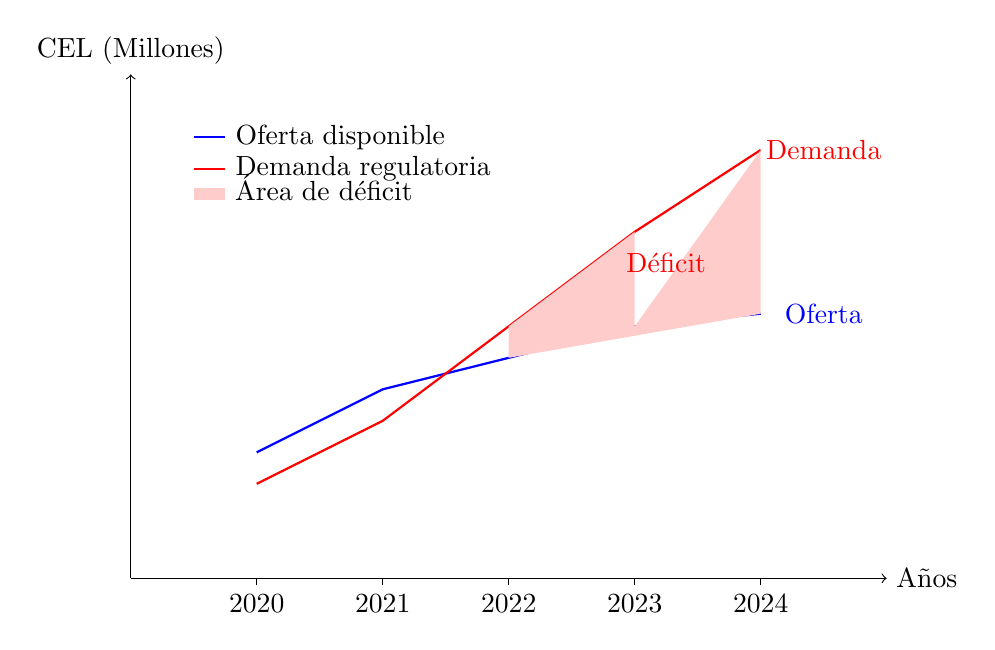
\begin{tikzpicture}[scale=0.8]
        % Ejes
        \draw[->] (0,0) -- (12,0) node[right] {Años};
        \draw[->] (0,0) -- (0,8) node[above] {CEL (Millones)};
        
        % Etiquetas de años
        \foreach \x/\year in {2/2020,4/2021,6/2022,8/2023,10/2024} {
            \draw (\x,0) -- (\x,-0.1) node[below] {\year};
        }
        
        % Línea de oferta (azul)
        \draw[thick, blue] (2,2) -- (4,3) -- (6,3.5) -- (8,4) -- (10,4.2);
        \node[blue] at (11,4.2) {Oferta};
        
        % Línea de demanda (rojo)
        \draw[thick, red] (2,1.5) -- (4,2.5) -- (6,4) -- (8,5.5) -- (10,6.8);
        \node[red] at (11,6.8) {Demanda};
        
        % Área de déficit
        \fill[red!20] (6,3.5) -- (6,4) -- (8,5.5) -- (8,4) -- (10,6.8) -- (10,4.2) -- cycle;
        \node[red] at (8.5,5) {Déficit};
        
        % Leyenda
        \draw[blue, thick] (1,7) -- (1.5,7) node[right, black] {Oferta disponible};
        \draw[red, thick] (1,6.5) -- (1.5,6.5) node[right, black] {Demanda regulatoria};
        \fill[red!20] (1,6) rectangle (1.5,6.2) node[right, black] {Área de déficit};
    \end{tikzpicture}
    \end{center}
    
    \fuenteHorizontal{Elaboración SENER con datos del S-CEL y reportes de cumplimiento de obligaciones}
\end{figuraespecial}

\subsection{Estado objetivo}

Establecer un sistema de monitoreo en tiempo real de la disponibilidad de CEL que permita ajustes dinámicos.

\subsection{Tabla comparativa: modelo actual vs modelo objetivo}

\subsection{Arquitectura del sistema (alto nivel)}

\subsection{Reingeniería de procesos (pasos operativos)}

\subsection{Beneficios esperados}

\subsection{Propuesta de ajuste normativo}

% =====================================================================
\section{Mecanismos de flexibilidad y diferimiento}

\subsection{Tabla de validación jurídica (interna)}

\subsection{Fuentes de información del S-CEL (obligatorio)}

\subsection{Diagnóstico de la situación actual}

Los mecanismos de flexibilidad actuales presentan limitaciones en su aplicación práctica.

\subsection{Estado objetivo}

Implementar mecanismos de flexibilidad más robustos y transparentes.

\subsection{Tabla comparativa: modelo actual vs modelo objetivo}

\subsection{Arquitectura del sistema (alto nivel)}

\subsection{Reingeniería de procesos (pasos operativos)}

\subsection{Beneficios esperados}

\subsection{Propuesta de ajuste normativo}

% =====================================================================
\section{Entidades voluntarias y cancelación voluntaria de Certificados}

\subsection{Tabla de validación jurídica (interna)}

\subsection{Fuentes de información del S-CEL (obligatorio)}

\subsection{Diagnóstico de la situación actual}

El mercado voluntario de CEL presenta oportunidades de desarrollo significativas.

\subsection{Estado objetivo}

Crear un mercado voluntario robusto que complemente las obligaciones regulatorias.

\subsection{Tabla comparativa: modelo actual vs modelo objetivo}

\subsection{Arquitectura del sistema (alto nivel)}

\subsection{Reingeniería de procesos (pasos operativos)}

\subsection{Beneficios esperados}

\subsection{Propuesta de ajuste normativo}

% =====================================================================
% BLOQUE IV · MECANISMOS DE TRANSACCIÓN
% =====================================================================

% Portada de sección para Bloque IV
\portadaseccion{IV}{Mecanismos de Transacción}{Mercado de CEL y transacciones bilaterales}

\section{Mercado de Certificados de Energía Limpia y transacciones bilaterales}

\subsection{Tabla de validación jurídica (interna)}

\subsection{Fuentes de información del S-CEL (obligatorio)}

\subsection{Diagnóstico de la situación actual}

El mercado bilateral de CEL requiere mayor transparencia y eficiencia.

\subsection{Estado objetivo}

Desarrollar un mercado transparente y eficiente para transacciones de CEL.

\subsection{Tabla comparativa: modelo actual vs modelo objetivo}

\subsection{Arquitectura del sistema (alto nivel)}

\subsection{Reingeniería de procesos (pasos operativos)}

\subsection{Beneficios esperados}

\subsection{Propuesta de ajuste normativo}

% =====================================================================
\section{Bolsa No Onerosa de Certificados de Energía Limpia}

\subsection{Tabla de validación jurídica (interna)}

\subsection{Fuentes de información del S-CEL (obligatorio)}

\subsection{Diagnóstico de la situación actual}

La Bolsa No Onerosa presenta distorsiones en las señales de mercado.

\subsection{Estado objetivo}

Reformar o eliminar la Bolsa No Onerosa para mejorar la eficiencia del mercado.

\subsection{Tabla comparativa: modelo actual vs modelo objetivo}

\subsection{Arquitectura del sistema (alto nivel)}

\subsection{Reingeniería de procesos (pasos operativos)}

\subsection{Beneficios esperados}

\subsection{Propuesta de ajuste normativo}

% =====================================================================
% BLOQUE V · PRECIO Y SEÑALES AMBIENTALES
% =====================================================================

% Portada de sección para Bloque V
\portadaseccion{V}{Precio y Señales Ambientales}{Formación de precios y factor de emisiones}

\section{Formación del precio del CEL y relación con el factor de emisiones}

\subsection{Tabla de validación jurídica (interna)}

\subsection{Fuentes de información del S-CEL (obligatorio)}

Incluir: Avisos de Factor de Emisión del SEN y fundamento regulatorio aplicable.

\subsection{Diagnóstico de la situación actual}

La formación de precios de CEL carece de transparencia y referencias claras.

\subsection{Estado objetivo}

Establecer mecanismos transparentes de formación de precios vinculados al factor de emisiones.

\subsection{Tabla comparativa: modelo actual vs modelo objetivo}

\subsection{Arquitectura del sistema (alto nivel)}

\subsection{Reingeniería de procesos (pasos operativos)}

\subsection{Beneficios esperados}

\subsection{Propuesta de ajuste normativo}

% =====================================================================
% BLOQUE VI · INSTRUMENTOS DE MEDIANO Y LARGO PLAZO
% =====================================================================

% Portada de sección para Bloque VI
\portadaseccion{VI}{Instrumentos de Mediano y Largo Plazo}{Contratos de cobertura y subastas}

\section{Certificados de Energía Limpia en contratos de cobertura}

\subsection{Tabla de validación jurídica (interna)}

\subsection{Fuentes de información del S-CEL (obligatorio)}

\subsection{Diagnóstico de la situación actual}

Los contratos de cobertura requieren mayor claridad en la asignación de obligaciones de CEL.

\subsection{Estado objetivo}

Establecer marcos contractuales claros para la cobertura de obligaciones de CEL.

\subsection{Tabla comparativa: modelo actual vs modelo objetivo}

\subsection{Arquitectura del sistema (alto nivel)}

\subsection{Reingeniería de procesos (pasos operativos)}

\subsection{Beneficios esperados}

\subsection{Propuesta de ajuste normativo}

% =====================================================================
\section{Subastas de Certificados de Energía Limpia como instrumento de planeación (actualmente suspendidas)}

\subsection{Tabla de validación jurídica (interna)}

\subsection{Fuentes de información del S-CEL (obligatorio)}

Incluir: Manuales de Subastas y Bases del Mercado aplicables (histórico), y referencia a su suspensión (si aplica).

\subsection{Diagnóstico de la situación actual}

Las subastas de CEL están suspendidas, limitando los instrumentos de planeación a largo plazo.

\subsection{Estado objetivo}

Evaluar la reactivación de subastas como instrumento de planeación energética.

\subsection{Tabla comparativa: modelo actual vs modelo objetivo}

\subsection{Arquitectura del sistema (alto nivel)}

\subsection{Reingeniería de procesos (pasos operativos)}

\subsection{Beneficios esperados}

\subsection{Propuesta de ajuste normativo}

% =====================================================================
% BLOQUE VII · CUMPLIMIENTO, SANCIÓN Y TRANSPARENCIA
% =====================================================================

% Portada de sección para Bloque VII
\portadaseccion{VII}{Cumplimiento, Sanción y Transparencia}{DECLARACEL, sanciones y transparencia}

\section{DECLARACEL, liquidaciones y reliquidaciones}

\subsection{Tabla de validación jurídica (interna)}

\subsection{Fuentes de información del S-CEL (obligatorio)}

\subsection{Diagnóstico de la situación actual}

El sistema DECLARACEL presenta oportunidades de mejora en eficiencia y transparencia.

\subsection{Estado objetivo}

Modernizar DECLARACEL para mayor eficiencia y reducción de errores.

\subsection{Tabla comparativa: modelo actual vs modelo objetivo}

\subsection{Arquitectura del sistema (alto nivel)}

\subsection{Reingeniería de procesos (pasos operativos)}

\subsection{Beneficios esperados}

\subsection{Propuesta de ajuste normativo}

% =====================================================================
\section{Régimen de sanciones y señales regulatorias}

\subsection{Tabla de validación jurídica (interna)}

\subsection{Fuentes de información del S-CEL (obligatorio)}

\subsection{Diagnóstico de la situación actual}

El régimen sancionador actual presenta desafíos en su aplicación efectiva.

\subsection{Estado objetivo}

Establecer un régimen sancionador más eficaz y proporcional.

\subsection{Tabla comparativa: modelo actual vs modelo objetivo}

\subsection{Arquitectura del sistema (alto nivel)}

\subsection{Reingeniería de procesos (pasos operativos)}

\subsection{Beneficios esperados}

\subsection{Propuesta de ajuste normativo}

% =====================================================================
\section{Transparencia, información pública y reportes del mercado de CEL}

\subsection{Tabla de validación jurídica (interna)}

\subsection{Fuentes de información del S-CEL (obligatorio)}

\subsection{Diagnóstico de la situación actual}

La transparencia del mercado de CEL requiere mejoras significativas.

\subsection{Estado objetivo}

Implementar un sistema de transparencia integral para el mercado de CEL.

\subsection{Tabla comparativa: modelo actual vs modelo objetivo}

\subsection{Arquitectura del sistema (alto nivel)}

\subsection{Reingeniería de procesos (pasos operativos)}

\subsection{Beneficios esperados}

% =====================================================================
% GLOSARIO Y BIBLIOGRAFÍA
% =====================================================================

\section*{Glosario}
\addcontentsline{toc}{section}{Glosario}

\subsection*{Términos Técnicos}

\begin{description}
    \item[CEL (Certificado de Energía Limpia):] Título que acredita que una unidad de energía eléctrica fue generada por una Central Eléctrica Limpia.
    \item[S-CEL:] Sistema de Gestión de Certificados y Cumplimiento de Obligaciones de Energías Limpias.
    \item[Participante Obligado:] Suministrador o Usuario Calificado que debe cumplir con los requisitos de adquisición de CEL.
    \item[Generación Limpia Distribuida (GLD):] Generación de energía eléctrica a partir de Energías Limpias conectada en el Sistema Eléctrico de Distribución.
    \item[Dictamen Técnico:] Documento emitido por una Unidad de Inspección que certifica el cumplimiento de requisitos técnicos.
    \item[Unidad Acreditada:] Organismo de inspección acreditado para emitir dictámenes técnicos.
\end{description}

\subsection*{Términos Regulatorios}

\begin{description}
    \item[DACG:] Disposiciones Administrativas de Carácter General.
    \item[CNE:] Comisión Nacional de Energía.
    \item[CENACE:] Centro Nacional de Control de Energía.
    \item[SENER:] Secretaría de Energía.
    \item[LSE:] Ley del Sector Eléctrico.
\end{description}

\section*{Bibliografía}
\addcontentsline{toc}{section}{Bibliografía}

\begin{enumerate}
    \item Ley del Sector Eléctrico (2025). Diario Oficial de la Federación.
    \item Disposiciones Administrativas de Carácter General del Sistema de Gestión de Certificados y Cumplimiento de Obligaciones de Energías Limpias (RES/174/2016).
    \item Resolución por la que se establecen los criterios para el otorgamiento de Certificados de Energías Limpias (RES/1838/2016).
    \item NOM-017-CRE-2019, Norma Oficial Mexicana de medición de variables para determinar el porcentaje de energía libre de combustible.
    \item Manual del Sistema de Gestión de Certificados y Cumplimiento de Obligaciones de Energías Limpias.
\end{enumerate}

% Contraportada institucional
\contraportada[img/contraportada.png]{
Este documento presenta un análisis integral de las áreas de oportunidad identificadas en el Sistema de Certificados de Energía Limpia (S-CEL), con propuestas específicas para su modernización y optimización.

El análisis abarca desde los procesos de entrada al sistema hasta los mecanismos de cumplimiento y sanción, proporcionando una hoja de ruta para la transformación del S-CEL en un instrumento más eficiente, transparente y alineado con los objetivos de la transición energética nacional.

Las propuestas presentadas buscan fortalecer la soberanía energética de México y posicionar al país como líder en certificación de energías limpias en América Latina.
}

\end{document}